\section{Challenges derived from including mobile devices}\label{challenges_derived_from_mobile_devides}
TODO

\subsection{Network instability}
TODO

\subsection{Battery consumption}
TODO 

% https://link.springer.com/chapter/10.1007/978-3-642-21726-5_2

% https://dl.acm.org/doi/abs/10.1145/2494232.2466586?casa_token=GWHJWfUGBmIAAAAA:clpjbVelNJzekDYVk1HEq1kmZ-7VeQ785Kuq414PfNrjfy9wKZ-WPfjD-B_VgsNvdjAITqh_8coFVg

% https://ieeexplore.ieee.org/abstract/document/8930492

\subsection{Limited resources}
TODO

\subsection{Even greater focus on security}
\textbf{As the number of smartphone increases}, the number of computers used by people are gradually declining (\textit{figure \ref{fig:global_sales_of_pcs_and_smartphones}}); as a direct consequence of these phenomena, \textbf{malicious attack efforts are now being redirected to exploiting mobile devices' vulnerabilities}.
\begin{figure}[H]
    \centering
    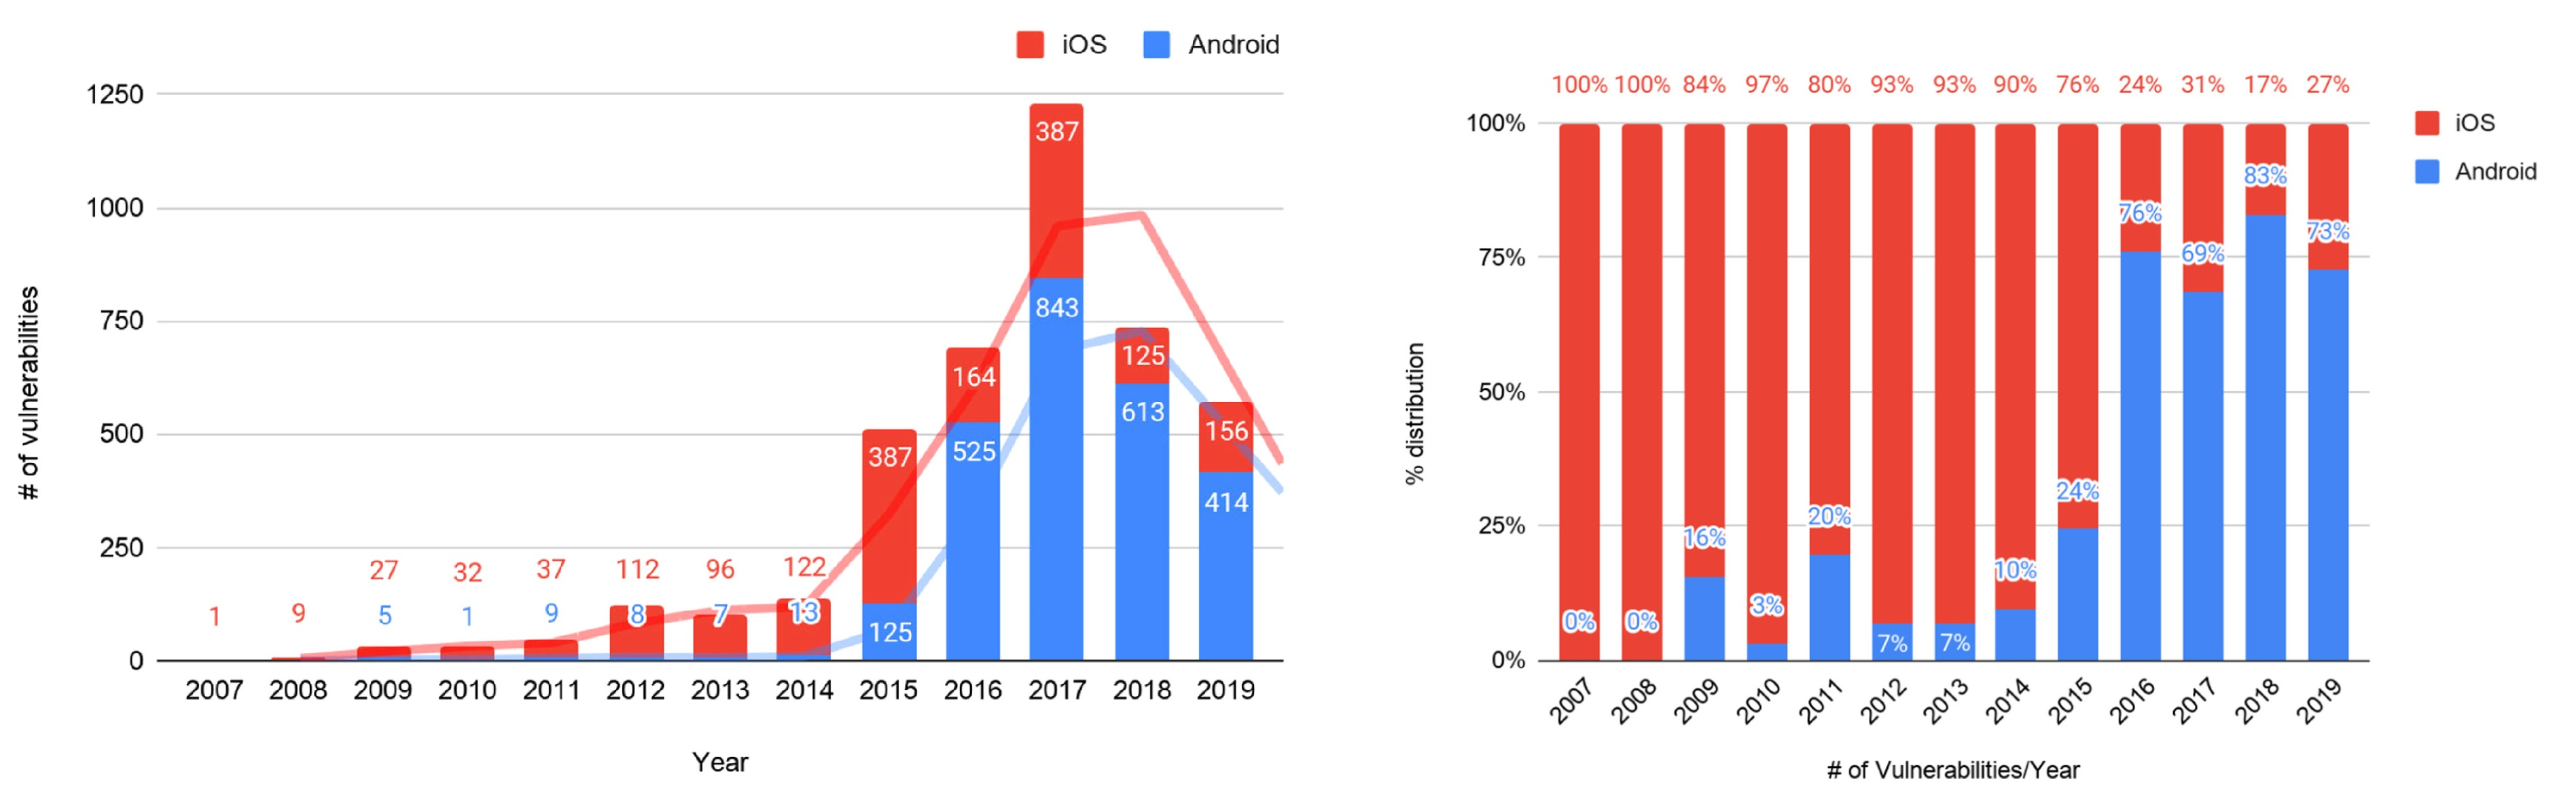
\includegraphics[width=\linewidth]{document/chapters/chapter_3/images/mobile_vulnerabilities.jpg}
    \caption{Number (left) and distribution (right) of known vulnerabilities on iOS and Android from 2007 to 2019 \cite{mobile_security}}
    \label{fig:mobile_vulnerabilities}
\end{figure}
\textit{Figure \ref{fig:mobile_vulnerabilities}} shows how \textbf{Android has more vulnerabilities compared to iOS}. This can be explained for the following two reasons:
\begin{itemize}
    \item \textbf{Android devices are more diffused}\\
    Attackers tend to attack these devices more since the pool of individual units is larger (as shown in \textit{image \ref{fig:os_market_share_2012_to_2021}}) and thus obtaining a profit is more likely.
    \item \textbf{iOS has more strict security measures} \cite{mobile_security}\\
    One of the byproducts of designing Android to be able to run a vast number of different hardware is the fact that compromises have to be made in order to grant compatibility. On the other hand, iOS runs on only a limited number of models, making it easier to design more effective security mechanisms. 
\end{itemize}
Through the \textbf{Linux Kernel}, Android resources are managed and protected. Furthermore, Android employs an \textbf{Application Sandbox} security mechanism, meaning that each application is run with a unique ID and the \textbf{processes are executed in spaces separated from each other and from the Kernel}, therefore preventing an application to interfere with the functioning of another. Despite this, Android employs an \textbf{authorization-based mechanism for accessing resources}; while \textbf{a process that has not the correct authorizations cannot access determinate resources}, the greatest weakness of this mechanism is the fact that \textbf{authorizations are granted by the user} which, usually, is not really aware of the implications of such choices. Application, consequently, can launch \textbf{various types of attacks depending on the type of authorizations} that they obtained. Another weakness of Android systems is the fact that \textbf{Application provenance is not guaranteed}; the Play Store's digital certificate can be easily obtained from malicious parties since Google only requires a fee paid by a credit card to get it (and payments might be done with a stolen credit card). Applications can also be installed from third parties, making it easier to introduce malicious software that is completely unchecked.

On the other hand, \textbf{iOS} utilizes a similar Sandbox system, but \textbf{authorizations are completely managed by the OS}, removing the possibility of human errors. From the Application provenance perspective, iOS' applications are only distributed by the App Store; developers have to register, pass a \textbf{vetting process} that evaluates the Application which, in case no harm is detected, is \textbf{digitally signed} and only then published on the store. This process makes more difficult the introduction of harmful applications.
\begin{figure}[H]
    \centering
    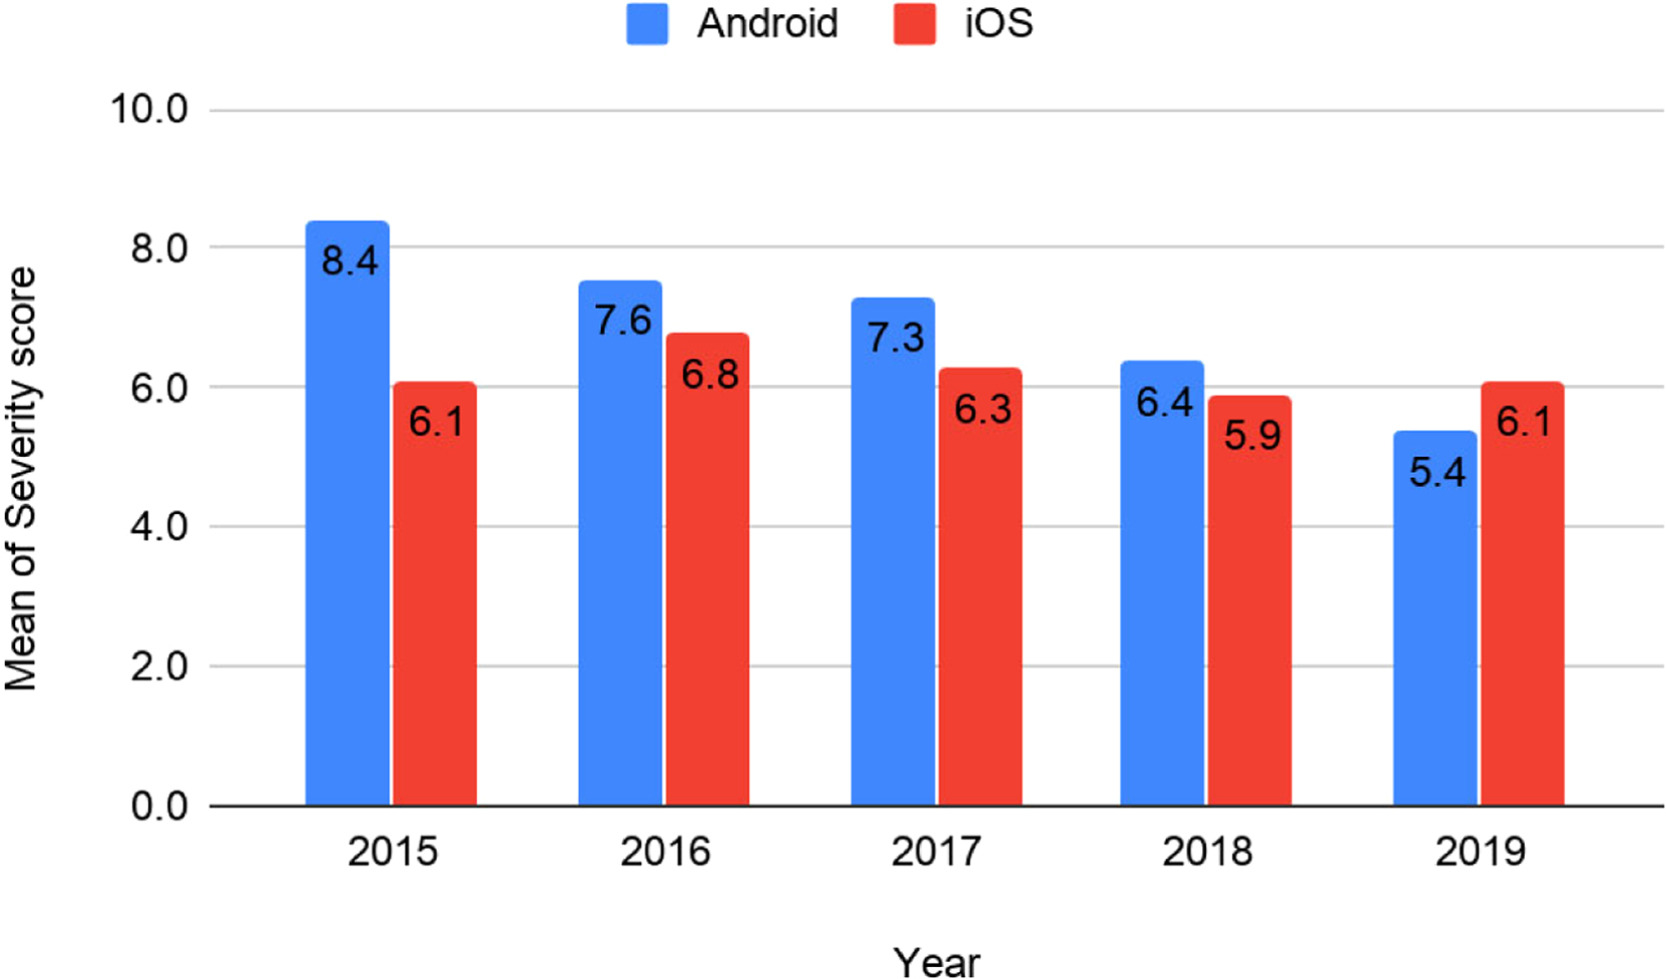
\includegraphics[scale=1.2]{document/chapters/chapter_3/images/mobile_vulnerabilities_severity.jpg}
    \caption{iOS and Android vulnerabilities severity score from 2015 to 2019 \cite{mobile_security}}
    \label{fig:mobile_vulnerabilities_severity}
\end{figure}
Even though iOS has the advantage when it comes to sheer number of security breaches, \textbf{with time the severity of Android's breached has decreased, becoming less severe than the iOS' ones} (\textit{figure \ref{fig:mobile_vulnerabilities_severity}}).

This data highlights how it is particularly important to focus on the security of the Grid's Fabric Layer (\textit{section \ref{fig:fabric_layer}}) while dealing with mobile devices because, in the current panorama, they are the greatest source of security vulnerabilities, especially considering that the information inside them has great value for attackers.

\subsection{Compatibility issues}
TODO
